\usepackage{graphicx}
\newenvironment{assgts}{%
  \renewcommand \labelenumi {\bfseries (\alph {enumi})}%
  \begin{enumerate}}{\end{enumerate}}
\let \super \textsuperscript
\newcommand \squoted [1]{‘#1’}
\newcommand \bord [1]{{\itshape\bfseries #1}}
\newcommand \word [1]{{\itshape #1}}
\newcommand \onor [1]{\bgroup #1\egroup}
\newcommand \onob [1]{\bgroup\bfseries #1\egroup}
\newcommand \trans [1]{\bgroup #1\egroup}
\newcommand \ipa [1]{\bgroup\bfseries #1\egroup}
\newcommand \chn [2]{\ipa{#1}$^{#2}$}
\newCJKfontfamily \ChnFont{Songti TC Light}
\newcommand \Ctx [1]{\bgroup\ChnFont#1\egroup}
\newcommand \Chn [3]{\Ctx{#1} \chn{#2}{#3}}
\newcommand \dql [2]{{\small #1}\quad \onob {#2}}
\newcommand \dqr [2]{{\small #1}\quad \onor {#2}}
\newcommand \gap [1]{\fbox{\normalfont \quad #1\quad}}
\newcommand \gzp [2]{$_{#1}$\fbox{\ #2\ }}
\def \dQ {\textsl{dróttkvætt}}
\newcommand \drotqone [4]{\nonlybut {#1}{#2}{#3 \et\ #4}. #3 \outother{#2}{#4}}
\newcommand \ts{c}
\newcommand \sz{ş}
\newcommand \cz{ç}
\newcommand \sj{\'x}
\newcommand \cj{k\llap{´}}
\newcommand \sibilants {\ipa{s} (\ipa{\ts}, \ipa{\ts{\super h}})}
\newcommand \retrofs {\ipa{\sz} (\ipa{\cz}, \ipa{\cz{\super h}})}
\newcommand \palatals {\ipa{\sj} (\ipa{\cj}, \ipa{\cj{\super h}})}
\newcommand \velars {\ipa{x} (\ipa{k}, \ipa{k{\super h}})}
\newcommand \nasals {\ipa m, \ipa n, \ipa{ŋ}}
\newcommand \picttone[1]{%
\begin{picture}(64,42)
\put(5,0){\makebox(0,0){\scriptsize 1}}
\put(5,10){\makebox(0,0){\scriptsize 2}}
\put(5,20){\makebox(0,0){\scriptsize 3}}
\put(5,30){\makebox(0,0){\scriptsize 4}}
\put(5,40){\makebox(0,0){\scriptsize 5}}
#1
\multiput(10,0)(0,10){4}{\dashbox{1}(50,10){}}
\end{picture}}
\newcommand \picttong[1]{%
\begin{picture}(30,22)
#1
\multiput(0,0)(0,5){4}{\dashbox{1}(30,5){}}
\end{picture}}
\newcommand \by [1]{%
  \unskip\nobreak\hfil\penalty50
  \hbox{}\nobreak\hfill{\hbox{\qquad\itshape #1}}\par}
\newsavebox {\tempobox}
\newlength\halftext
\halftext=\textwidth \advance \halftext by-50pt \divide \halftext by2

\makeatletter
\def \ps@somestyle {
      \let\@oddfoot\@empty
      \def\@oddhead{\textsl {\small \begin{tabular}[t]{@{}l}\pgheader\ (2008).\\ \chapname \end{tabular}}\hfill \thepage}}
\def\und@r#1#2{%
   {\oalign{#2\crcr\hidewidth
      \vbox to0ex{\hbox{#1}\vss}\hidewidth}}}
\def\rfx{\und@r{`}}
\makeatother

\def \problem {\stepcounter {section}\paragraph{\probword \thesection\ (20 \pontword).}}
\def \solution {\stepcounter {section}\paragraph{\probword \thesection.}}

\newcommand \makepart [1]{\newpage
\begin{center}%
{\LARGE \olympiad \par }
\vskip 1em{\begin{tabular}[t]{c}\Large \bulgaria, \sunbeach, \olydates
\end{tabular}\par }
\vskip 1em{\large #1}\end{center}\par \vskip .5em
\def \chapname {#1}\setcounter {section}0\setcounter {page}1}

\begin{document}
\hyphenation{Guang-yun}
\ifx\enumLat\undefined\else\enumLat\fi

\thispagestyle{empty}
\makepart{\probindl}

\pagestyle{somestyle}

\centerline{\textbf{\regulats}}
%
\begin{enumerate}
\item \regulatx. \towarrant
\item \regulaty
\end{enumerate}

\problem \inmicmac:

\medskip\centerline{\begin{tabular}{|r|l|l|l|}\hline
1 & \bord{tmi'gn} & \trans{dəmīgən} & \axeparol \\
2 & \bord{an'stawteg} & \trans{anəstawtek} & \unsafewd \\
3 & \bord{gjiansale'wit} & \trans{əkciansalēwit} & \arxangel \\
4 & \bord{mgumie'jo'tlatl} & \trans{əmkumiējōdəladəl} & \shoeword \\
5 & \bord{amqwanji'j} & \trans{amxʷancīc} & \spoonmot \\
6 & \bord{e'jnt} & \trans{ējənt} & \agentmot \\
7 & \bord{tplutaqan} & \trans{ətpəludaγan} & \lawparol \\
8 & \bord{ge'gwising} & \trans{gēgʷisink} & \lieontop \\
9 & \bord{lnu'sgw} & \trans{lənūskʷ} & \indianfe \\
10 & \bord{g'p'ta'q} & \trans{gəbədāx} & \abovemot \\
11 & \bord{epsaqtejg} & \trans{epsaxteck} & \stovemot \\ \hline
\end{tabular}}

\begin{assgts}
\item \transcri:

\medskip\centerline{\begin{tabular}{|r|l|l|}\hline
12 & \bord{gsnqo'qon} & \foolishn \\
13 & \bord{tg'poq} & \springwa \\
14 & \bord{gmu'jmin} & \raspberr \\
15 & \bord{emtoqwatg} & \worships \\
16 & \bord{te'plj} & \goatword \\ \hline
\end{tabular}}
%
\item \writorth:

\medskip\centerline{\begin{tabular}{|r|l|l|}\hline
17 & \trans{ətpədēsən} & \southmot \\
18 & \trans{əmteskəm} & \snakemot \\
19 & \trans{alaptək} & \lookroon \\
20 & \trans{gəlamen} & \therefor \\ \hline
\end{tabular}}
\end{assgts}
%
\textbf{NB:} \gemicmac. \spokenca{8000}{\incanada}.

\macschwa {\trans{ə}}, \cjmicmac {[c]}{[j]}, [x] \frivelar, \trans{γ} \dittovoi;
[ʷ] \nbsuperw. \hetteken~¯ \longmark.
%
\by{—\BBname}

\newpage

\problem \inscalds {\dQ}:
%
\begin{quote}
\parbox{\halftext}{\textbf{I}\smallskip \\
\dql1{ók at ísarnleiki} \\
\dql2{Jarðar sunr, en dunði …}\medskip \\
\textbf{II}\smallskip \\
%\dql1{fljótt bað foldar dróttinn}\\
%\dql2{Fárbauta mǫg Várar}\\
\dql1{þekkiligr með þegnum}\\
\dql2{þrymseilar hval deila.}\\
\dql3{en af breiðu bjóði}\\
\dql4{bragðvíss at þat lagði}\\
\dql5{ósvífrandi ása}\\
\dql6{upp þjórhluti fjóra.}}\hfill
\parbox{\halftext}{\textbf{III}\smallskip \\
\dql1{áðr gnapsólar Gripnis}\\
\dql2{gnýstœrandi fœri}\\
\dql3{rausnarsamr til rimmu}\\
\dql4{ríðviggs lagar skíðum.}\medskip \\
\textbf{IV}\smallskip \\
\dql1{háði gramr, þars gnúðu,} \\
\dql2{geira hregg við seggi,} \\
\dql3{(rauð fnýsti ben blóði)} \\
\dql4{bryngǫgl í dyn Skǫglar,} \\
\dql5{þás á rausn fyr ræsi} \\
\dql6{(réð egglituðr) seggir …}}
\end{quote}
%
\allitert {\dQ}. \alliterh: \eg\ \onob{rausnarsamr}, \onob{rimmu} \et\ \onob{ríðviggs} (III:3–4).
\vocallit {\onob{j}}: \eg\ \onob{ók}, \onob{ísarnleiki} \et\ \onob{Jarðar} (I:1–2). \nunirule.

\mdiffers. \mvariats. \huchoose.
\drotqone {I:2}{\onob{dunði}}{\onob{dulði}}{\onob{djarfi}}
\drotqtri {III:1}{\onob{Gripnis}}{\onob{Grímnis}}

\begin{assgts}
\item \vadrules {\dQ}.

\bigskip\centerline{***}

\item \dqstanza:
%
\medskip \\
\parbox{170pt}{\textbf{V}\smallskip \\
\dql1{\gap a (þreifsk reiddra øxa} \\
\dql2{\gap b ; knǫ́ttu spjǫ́r \gap c )} \\
\dql3{\gap d bitu seggi} \\
\dql4{\gap e þjóðkonungs ferðar,} \\
\dql5{þás ( \gap f hǫlða)} \\
\dql6{\gap g \gap h \gap i} \\
\dql7{(hǫ́r vas \gap j of \gap k )} \\
\dql8{\gap l (flugbeiddra \gap m ).}}\hfill
\parbox{200pt}{\dqfiller:
\begin{quote}
\onob{andskoti, Gauta, glymja, hlaut, hugfyldra, hœgra, ríks, rymr, sigr, smíði, svartskyggð, sverð, svírum, sǫngr, vigra}
\end{quote}
%
\fillgaps.}
%
\end{assgts}
\textbf{NB:} \wwonorse.

\onororth {\onob{æ}}{\onob{œ}}{\onob{ø}}; \onob{y} \uyumlaut, \onob{ǫ} \oshiroko.
\onob{au} \et\ \onob{ei} \singsyll.
\ifx\jotisjot nay\onob{j} \jotsound.\fi
{\onob{ð} \et\ \onob{þ}} = \thorneth {\word{th}}{\word{this}}{\word{thin}}.
\onob{x} = \onob{k}+\onob{s}. \hetteken~´ \longmark. \onornorm.
\by{—\APname}

\newpage

\problem \indrecem\ -- \drehname\et\cemuname
\ -- \et\theirtra\chaotict:

\savebox {\tempobox}{\itshape\bfseries ngöne-uma, nyine-thin, uma-hmitrötr}
\newlength \ritewide
\ritewide=\textwidth \advance \ritewide by-\wd\tempobox
\advance \ritewide by-50pt

\medskip\centerline{\begin{tabular}{|l|l|}\hline
\drehname & \thisling \\ \hline
\parbox{\wd\tempobox}{\itshape\bfseries\raggedright\smallskip
drai-hmitrötr, gaa-hmitrötr, i-drai, \mbox{i-jun}, i-wahnawa, jun, ngöne-gejë, ngöne-uma, nyine-thin, uma-hmitrötr}
&
\parbox{\ritewide}{\raggedright \autelmot, \bananasz, \calendar, \boneword, \ecclesia, \costemot, \carrelet, \dimanche, \skeleton, \murparol}\\ \hline
\end{tabular}}

\medskip\centerline{\begin{tabular}{|l|l|}\hline
\cemuname & \thisling \\ \hline
\parbox{\wd\tempobox}{\itshape\bfseries\raggedright
a-pulut, ba-bwén, ba-jié, bé-ôdu, bé-tii, bé-wöli, bé-wöli-wöta, tii, wöta}
&
\parbox{\ritewide}{\raggedright\smallskip \litparol, \animalwd, \fourchet, \verremot, \kurkalem, \costemot, \schrimot, \twilight, \esperonx}\\ \hline
\end{tabular}}
\mbox{}\\
%
\redrecem {\drehname}{\cemuname}:
\medskip \\
%
\mbox{}\qquad \begin{tabular}{|l|l|l|l|l|}\hline
\drehname & \bord{gaa} & \bord{ngöne-gejë} & \bord{nyine} & \bord{thin} \\ \hline
\cemuname & \bord{a} & \bord{ba-jié} & \bord{bé} & \bord{wöli} \\ \hline
\end{tabular}
%
\begin{assgts}
\item \corrcorr.\hfill
\raisebox{-2ex}[1ex][0ex]{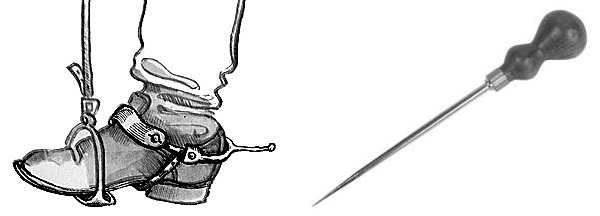
\includegraphics[bb = 0 0 600 216,scale=.25]{bothpixt.jpg}}\llap
{\begin{picture}(100,10)
\put(15,30){\small \esperonx}
\put(18,27){\vector(0,-1){15}}
\put(64,8){\small \carrelet}
\end{picture}}
\item \cdaskone{\bord{wahnawa} \et\ \bord{drai}}{\drehname}{\bord{wöli} \et\ \bord{pulut\/}}{\cemuname}?
\item \cdasktwo{\drehname}{\bord{tusi}}{\tomeword}{\bord{bii}}{\abeillex}.
\outdrehu{\drehname}: \bord{i-bii}, \bord{tusi-hmitrötr}.
\end{assgts}
%
{\small \textbf{NB:} \drehspok {10\,000}.
\cemuspok {2000}. \bothaune.

\indrehus\
\bord{ë} \eshiroko, \bord{ö} \owumlaut, \bord{hm} \et~\bord{hn} \spunvoid;
\bord{dr} \et~\bord{tr} \retrflex;
{\bord{j} \et\ \bord{th}} = \thorneth {\word{th}}{\word{this}}{\word{thin}};
\bord{ng} \velarnas; \bord{ny} \palatnas.

\autelexp.}
%
\by{—\XGname}

\problem \giveword {\zoquenom}\et\theirtra:\medskip

\centerline{\begin{tabular}{ll}
\ipa{mis nakpatpit} & \cutunakpat \\
\ipa{nakpat} & \nakpat \\
\ipa{mokpittih} & \solo\cumokmok \\
\ipa{pokskuky2sm2taPm} & \supoxkuys \\
\ipa{pokskuy} & \poxkuy \\
\ipa{peroltih} & \solo\kittel \\
\ipa{koc2ktaPm} & \balkanes \\
\ipa{komg2sm2tih} & \rite\supillar \\
\ipa{P2s ŋgom} & \mipillar \\
\ipa{k2m2ŋbitšeh} & \cosi\cushadow \\
\end{tabular}
\begin{tabular}{ll}
\ipa{k2m2ŋdaPm} & \shadows \\
\ipa{P2s ncapk2sm2šeh} & \cosi\sumihimmel \\
\ipa{capšeh} & \como\himmel \\
\ipa{pahsungotoya} & \zacourge \\
\ipa{pahsunšehtaPmdih} & \just\como\courges \\
\ipa{t2ckotoyatih} & \solo\zadiente \\
\ipa{kumguky2sm2} & \sukumguy \\
\ipa{kumgukyotoyataPm} & \zakumguys \\
\ipa{cakyotoya} & \zacaycay \\
\ipa{mis ncay} & \tucaycay \\
\end{tabular}}\mbox{}\medskip \\
\quad
\parbox{\halftext}{\textbf{(a)} \fordinto {\thislang}:
\begin{quote}
\ipa{caky2sm2tih} \\
\ipa{k2m2ŋšeh} \\
\ipa{P2s mok} \\
\ipa{mis nd2ctaPm} \\
\ipa{pahsunbit} \\
\ipa{perolkotoyašehtaPm}
\end{quote}}\hfill
\parbox{\halftext}{\textbf{(b)} \fordinto {\zoquenom}:
\begin{quote}
\zapoxkuy \\
\cumikittel \\
\just\como\balkan \\
\pillars \\
\sushadows \\
\tukumguy
\end{quote}} \\
%
\textbf{NB:} \genzoque {\zoquenom}. \spokenca {10\,000}{\inchiapa}.

\ipa{2} \zoqwedge;
{\ipa{c}} \tsaffric, \zoqconsz {\ipa{nc}}{\ipa{š}}, \ipa{ŋ}~\velarnas, \ipa{y} \jotsound; \ipa{P}~\glotstop.
%
\by{—\IDname}

\problem \insentin {\inukname}\et\theirtra:\medskip \\
%
\begin{tabular}{rll}
1. & \bord{Qingmivit takujaatit.} & \sinukoer\inuktitb. \\
2. & \bord{Inuuhuktuup iluaqhaiji qukiqtanga.} & \inuktitf. \\
3. & \bord{Aanniqtutit.} & \inuktitl. \\
4. & \bord{Iluaqhaijiup aarqijaatit.} & \inuktita. \\
5. & \bord{Qingmiq iputujait.} & \inuktitc. \\
6. & \bord{Angatkuq iluaqhaijimik aarqisijuq.} & \deshaman\inuktitj. \\
7. & \bord{Nanuq qaijuq.} & \inuktith. \\
8. & \bord{Iluaqhaijivit inuuhuktuit aarqijanga.} & \inuktitd. \\
9. & \bord{Angunahuktiup amaruq iputujanga.} & \thejager\inuktitg. \\
10. & \bord{Qingmiup ilinniaqtitsijiit aanniqtanga.} & \inuktite. \\
11. & \bord{Ukiakhaqtutit.} & \inuktitk. \\
12. & \bord{Angunahukti nanurmik qukiqsijuq.} & \thejager\inuktiti. \\
\end{tabular}
%
\begin{assgts}
\item \fordinto {\thislang}:

\begin{tabular}{rl}
13. & \bord{Amaruup angatkuit takujanga.} \\
14. & \bord{Nanuit inuuhukturmik aanniqsijuq.} \\
15. & \bord{Angunahuktiit aarqijuq.} \\
16. & \bord{Ilinniaqtitsiji qukiqtait.} \\
17. & \bord{Qaijutit.} \\
18. & \bord{Angunahuktimik aarqisijutit.} \\
\end{tabular}
\item \fordinto {\inukname}:

\begin{tabular}{rl}
19. & \deshaman\inuktits. \\
20. & \inuktitt. \\
21. & \inuktitu. \\
22. & \shottest{\adogword}. \\
23. & \sinukoer\inuktitw. \\
\end{tabular}
\end{assgts}
%
\textbf{NB:} \geninukt. \spokenca {35\,000}{\northcan}.

\rquvular {\bord{r}}{\bord{q}}.
\ifx\jotisjot nay\bord{j} \jotsound.\fi

\shamanex.
%
\by{—\BBname}

\vfill
\begin{center}
\textbf{\editorsz:} \edinames.\medskip

\textbf{\thistext:} \whowroti.\medskip

\large \goodluck!
\end{center}

\makepart{\solsindl}
\thispagestyle{empty}

\pagestyle{somestyle}
%
\solution \rulesmot:
%
\begin{enumerate}
\item \apostrof {\trans{ə}}.
\item \ruleforw {\bord{w}}{[w]}.
\item \trans{ə} \schwason {([l~m~n])}.
\item \trans{ə} \schwabis.
\item \rulestop{\bord{p t j g gw q qw}}{\trans{b d j g gʷ γ γʷ}}{\trans{p t c k kʷ x xʷ}}.
\end{enumerate}
%
\answersp:
%
\begin{assgts}
\item 12 \trans{əksənxōγon}, 13 \trans{ətkəbox}, 14 \trans{gəmūjəmin}, 15 \trans{emtoγʷatk}, 16 \trans{dēbəlc};
\item 17 \bord{tp'te'sn}, 18 \bord{mtesgm}, 19 \bord{alapt'g}, 20 \bord{glamen}.
\end{assgts}

\savebox {\tempobox}{\begin{tabular}{l@{}}
\textbf{V}\smallskip \\
\dqr1{\gzp a{\textbf rí\underline{ks}} (þreifsk \textbf reiddra ø\underline xa} \\
\dqr2{\gzp b{\textbf r\underline{ym}r} ; knǫ́ttu spjǫ́r \gzp c{gl\underline{ym}ja} )} \\
\dqr3{\gzp d{\textbf svartsky\underline{gg}ð} bitu \textbf se\underline{gg}i} \\
\dqr4{\gzp e{\textbf sv\underline{erð}} þjóðkonungs f\underline{erð}ar,} \\
\dqr5{þás ( \gzp f{\textbf hugfy\underline ldra} \textbf hǫ\underline lða)} \\
\dqr6{\gzp g{\textbf hl\underline{aut}} \gzp h{andskoti} \gzp i{G\underline{aut}a}} \\
\dqr7{(hǫ́\underline r vas \gzp j{\textbf sǫngr} of \gzp k{\textbf sví\underline rum} )} \\
\dqr8{\gzp l{\textbf s\underline{igr}} (flugbeiddra \gzp m{v\underline{igr}a} ).}
\end{tabular}}
\newlength \motiwide
\motiwide=\textwidth
\advance \motiwide by-\wd\tempobox
\advance \motiwide by-2em

\solution \textbf{(a)} \rulesmot:
%
\begin{itemize}
\item[1.] \qtysylla.
\item[2.] \allitera. \videstat.
\item[3.] \inrhymes.
\inrhymep\ V$_1$, V$_2$, …, V$_6$. \inrhymeq {V$_n$}{($n$ = 1, 2 \au~3)}. \inrhymer\ V$_n$ = V$_5$.
\end{itemize}
%\bigskip \\
%
\begin{minipage}{\motiwide}
\egdrotts {IV, 1–6}:
\begin{quote}
\textbf{IV}\smallskip \\
\dqr1{há\underline{ð}i \textbf gramr, þars \textbf gnú\underline{ð}u,} \\
\dqr2{\textbf geira hr\underline{egg} við s\underline{egg}i,} \\
\dqr3{(rau\underline{ð} fnýsti \textbf ben \textbf bló\underline{ð}i)} \\
\dqr4{\textbf bryng\underline{ǫgl} í dyn Sk\underline{ǫgl}ar,} \\
\dqr5{þás á \textbf rau\underline sn fyr \textbf ræ\underline si} \\
\dqr6{(\textbf réð \underline{egg}lituðr) s\underline{egg}ir …}
\end{quote}
\textbf{(b)} \excesswd: \onob{hœgra}, \onob{smíði}.
\end{minipage}
\hfill \usebox {\tempobox}

\solution \cedreord.
%
\begin{assgts}
\item
\begin{tabular}[t]{lll}
\bord{jun} & \boneword \\
\bord{i-jun} & \skeleton & (\multitud {\bonemult}) \\
\bord{i-wahnawa} & \bananasz & (\multitud {\banamult}) \\
\bord{i-drai} & \calendar & (\multitud {\jourmult}) \\	
\bord{drai-hmitrötr} & \dimanche & (\holyjour\jourword) \\
\bord{gaa-hmitrötr} & \autelmot & (\holypost\postword) \\
\bord{uma-hmitrötr} & \ecclesia & (\holyhome\homeword) \\
\bord{ngöne-uma} & \murparol & (\frontier {\homegran}) \\
\bord{ngöne-gejë} & \costemot & (\frontier {\aquagran}) \\
\bord{nyine-thin} & \carrelet & (\tool {\piquemis}) \\\hline
\bord{tii} & \schrimot \\
\bord{bé-tii} & \kurkalem & (\tool {\schrimis}) \\
\bord{bé-wöli} & \fourchet & (\tool {\piquemis}) \\
\bord{wöta} & \animalwd \\
\bord{bé-wöli-wöta} & \esperonx & (\esperony) \\
\bord{bé-ôdu} & \verremot & (\tool {\boiremis}) \\
\bord{ba-jié} & \costemot & (\frontier {\aquagran}) \\
\bord{ba-bwén} & \twilight & (\frontier {\nuitgran}) \\
\bord{a-pulut} & \litparol & (\postdorm) \\
\end{tabular}
\item \bord{wahnawa} \squoted{\bananawd}, \bord{drai} \squoted{\jourword}; \bord{wöli} \squoted{\piquemot}, \bord{pulut} \squoted{\dormimot}.
\item \bord{i-bii} \squoted{\abeilles\ (\multitud {\abeimult})}, \bord{tusi-hmitrötr} \squoted{\biblemot\ (\holytome\tomeword)}.
\end{assgts}

\solution \zoquesfx:
%
\begin{enumerate}
\item \ipa{-k2sm2} \squoted{\abovemot}, \ipa{-kotoya} \squoted{\forparol}, \ipa{-pit} \withword;
\item \ipa{-šeh} \squoted{\como, \cosi};
\item \ipa{-taPm} \renderpl;
\item \ipa{-tih} \squoted{\solo\ (\just, \rite)}.
\end{enumerate}
%
\simnasal {\nasals}{\ipa p, \ipa t, \ipa k}{\ipa b, \ipa d, \ipa g}.
\metathyk {\ipa k}{\ipa y}.

\possezoq {\ipa{P2s}}{\ipa{mis}};
\prenasal.
%
\begin{assgts}
\item
\begin{tabular}[t]{ll}
\ipa{caky2sm2tih} & \rite\sucaycay \\
\ipa{k2m2ŋšeh} & \como\shadow \\
\ipa{P2s mok} & \mimokmok \\
\ipa{mis nd2ctaPm} & \tudientes \\
\ipa{pahsunbit} & \cucourge \\
\ipa{perolkotoyašehtaPm} & \cosi\zakittels \\
\end{tabular}
\item
\begin{tabular}[t]{ll}
\zapoxkuy & \ipa{pokskukyotoya} \\
\cumikittel & \ipa{P2s mberolpit} \\
\just\como\balkan & \ipa{koc2kšehtih} \\
\pillars & \ipa{komdaPm} \\
\sushadows & \ipa{k2m2ŋg2sm2taPm} \\
\tukumguy & \ipa{mis ŋgumguy} \\
\end{tabular}
\end{assgts}

\solution \instruct:\medskip \\
%
\begin{tabular}{l@{\quad }l@{\quad }l@{\quad }l|l}
& \textsf{X}-\bord{(q)} && \textsf{V}-- & \squoted{\textsf{X} \Vhimself.} \\
& \textsf{X}-\bord{(q)} & \textsf{Y}-\bord{(r)mik} & \textsf{V}-\bord{si}-- & \squoted{\textsf{X} \textsf{V} \aYrender.} \\
\textsf{X}-\bord{up} & \textsf{Y}-\bord{(q)} && \textsf{V}-- & \squoted{\textsf{X} \textsf{V} \theYrend.} \\
\end{tabular}
\medskip \\
%
\wherinuk {\textsf{X} \et\ \textsf{Y}}{\textsf{V}}.
\declinuk {\mbox{\bord{-q}}}{\bord{-r}}{\bord{-mik}}
(\bord{nanu-q} — \bord{nanu-r-mik}; \bord{iluaqhaiji} — \bord{iluaqhaiji-mik}).
\sayyours {\bord{-(q)}}{\bord{-it}}{\bord{-up}}{\bord{-vit}}.

\suffinuk:
%
\begin{itemize}
\item \jortinuk {\bord{-j}}{\bord{-t}};
\item \endingin:
\begin{itemize}
\item \schemata: \bord{-u-tit} \squoted{2}, \bord{-u-q} \squoted{3};
\item \schematr: \bord{-a-it} \squoted{2/3}, \bord{-a-nga} \squoted{3/3}, \bord{-a-atit} \squoted{3/2}.
\end{itemize}
\end{itemize}
%
\transref.
%
\begin{assgts}
\item
\begin{tabular}[t]{rll}
13. & \inuktitm. \\
14. & \inuktitn. \\
15. & \inuktito. \\
16. & \shottest{\tteacher}. \\
17. & \inuktitq. \\
18. & \inuktitr. \\
\end{tabular}
%
\item
\begin{tabular}[t]{rll}
19. & \bord{Angatkuup aanniqtaatit.} \\
20. & \bord{Ilinniaqtitsijiup inuuhuktuq takujanga.} \\
21. & \bord{Amaruit ukiakhaqtuq.} \\
22. & \bord{Qingmirmik qukiqsijutit.} \\
23. & \bord{Qingmiit ilinniaqtitsijimik aanniqsijuq.} \\
\end{tabular}
\end{assgts}

\makepart{\probteam}
\thispagestyle{empty}

\pagestyle{somestyle}

\homochin {\Guangyun}{1007--1011}. \nophonet, \oneastwo. \calledfq

\hetechin

\herecant \medskip \\
%
\begin{tabular}{rl@{ = }l@{ $\star$ }l}
& \xarakter & \multicolumn{2}{c}{\transcrn} \\\hline
1. & \Chn{倦}{kyn}{2} & \Chn{渠}{k\super hœy}{21} & \Chn{卷}{kyn}{3}\\
2. & \Chn{求}{k\super hau}{21} & \Chn{巨}{kœy}{2} & \Chn{鳩}{kau}{53}\\
3. & \Chn{住}{{\ts}y}{2} & \Chn{持}{{\ts}\super hi}{21} & \Chn{遇}{y}{2}\\
4. & \Chn{病}{piŋ}{2} & \Chn{皮}{p\super hei}{21} & \Chn{命}{miŋ}{2}\\
5. & \Chn{掉}{tiu}{2} & \Chn{徒}{t\super hou}{21} & \Chn{弔}{tiu}{3}\\
6. & \Chn{鳩}{kau}{53} & \Chn{居}{kœy}{53} & \Chn{求}{k\super hau}{21}\\
7. & \Chn{僖}{hei}{53} & \Chn{許}{hœy}{35} & \Chn{其}{k\super hei}{21}\\
8. & \Chn{朗}{loŋ}{13} & \Chn{盧}{lou}{21} & \Chn{黨}{toŋ}{35}\\
9. & \Chn{韶}{siu}{21} & \Chn{市}{si}{13} & \Chn{昭}{{\ts}iu}{53}\\
10. & \Chn{帳}{{\ts}œŋ}{3} & \Chn{知}{{\ts}i}{3} & \Chn{亮}{lœŋ}{2}\\
11. & \Chn{愀}{{\ts}\super hiu}{35} & \Chn{親}{{\ts}\super han}{3} & \Chn{小}{siu}{35}\\
12. & \Chn{舞}{mou}{13} & \Chn{文}{man}{2} & \Chn{甫}{p\super hou}{35}\\
13. & \Chn{謏}{siu}{35} & \Chn{先}{sin}{53} & \Chn{鳥}{niu}{13}\\
14. & \Chn{臼}{k\super hau}{13} & \Chn{其}{k\super hei}{21} & \Chn{九}{kau}{35}\\
15. & \Chn{斜}{{\ts}\super he}{21} & \Chn{似}{{\ts}\super hi}{13} & \Chn{嗟}{{\ts}e}{53}\\
16. & \Chn{冓}{kau}{3} & \Chn{古}{ku}{35} & \Chn{候}{hau}{2}\\
\end{tabular}
%
\begin{assgts}
\item \hucanton.
\item \huwasuse {\whencomp {\Guangyun}}? \whatonly {\incanton}
\end{assgts}
%
\nownovoi {\ipa l, \nasals}. \ccvoiced {\Guangyun}:
\devofric {\fromvoid}{\tounvoid} (\eg\ \ipa{z} \textgreater~\ipa{s}),
\devostop {\fromvoid}{\tounvoid} (\eg\ \ipa{d} \textgreater\ \ipa{t} \au~\ipa{t\super h}).
\wuvoiced. \wuvoicex{\Ctx{徒}}{[\chn{du}{21}]}{[\chn{t\super hou}{21}]}{[\chn{t\super hu}{35}]}.
%
\begin{assgts}\setcounter{enumi}2
\item \wherevoi {\whencomp {\Guangyun}}? \whyvdasp 
\item \tredecar. \hutresex
\end{assgts}
%
\heremand:\medskip \\
%
\begin{tabular}{rl@{ = }l@{ $\star$ }l}
17. & \Chn{邅}{{\cz}an}{5} & \Chn{張}{{\cz}aŋ}{5} & \Chn{連}{lian}{35} \\
18. & \Chn{良}{liaŋ}{35} & \Chn{呂}{ly}{214} & \Chn{章}{{\cz}aŋ}{5} \\
19. & \Chn{遵}{{\ts}un}{5} & \Chn{將}{{\cj}iaŋ}{51} & \Chn{倫}{lun}{35} \\
20. & \Chn{蕭}{{\sj}iao}{5} & \Chn{蘇}{su}{5} & \Chn{彫}{tiao}{5} \\
21. & \Chn{嵌}{{\cj}\super hian}{5} & \Chn{口}{k\super hou}{214} & \Chn{銜}{{\sj}ian}{35} \\
22. & \Chn{先}{{\sj}ian}{5} & \Chn{蘇}{su}{5} & \Chn{前}{{\cj}\super hian}{35} \\
23. & \Chn{巉}{{\cz}\super han}{35} & \Chn{鋤}{{\cz}\super hu}{35} & \Chn{銜}{{\cj}\super hian}{35} \\
24. & \Chn{婞}{{\sj}iŋ}{51} & \Chn{胡}{xu}{35} & \Chn{頂}{tiŋ}{214} \\
25. & \Chn{丳}{{\cz}\super han}{214} & \Chn{初}{{\cz}\super hu}{5} & \Chn{限}{{\sj}ian}{51} \\
26. & \Chn{趡}{{\ts}\super huei}{214} & \Chn{千}{{\cj}\super hian}{5} & \Chn{水}{{\sz}uei}{214} \\
27. & \Chn{初}{{\cz}\super hu}{5} & \Chn{楚}{{\cz}\super hu}{214} & \Chn{居}{{\cj}y}{5} \\
28. & \Chn{釧}{{\cz}\super huan}{51} & \Chn{尺}{{\cz}\super h\,}{214} & \Chn{絹}{{\cj}yan}{51} \\
29. & \Chn{卷}{{\cj}yan}{214} & \Chn{居}{{\cj}y}{5} & \Chn{轉}{{\cz}uan}{214} \\
30. & \Chn{處}{{\cz}\super hu}{51} & \Chn{昌}{{\cz}\super haŋ}{5} & \Chn{據}{{\cj}y}{51} \\
31. & \Chn{俜}{p\super hiŋ}{5} & \Chn{普}{p\super hu}{214} & \Chn{丁}{tiŋ}{5} \\
32. & \Chn{蚪}{tou}{214} & \Chn{當}{taŋ}{5} & \Chn{口}{k\super hou}{214} \\
\end{tabular}
%
\begin{assgts}\setcounter{enumi}4
\item \formanda
\end{assgts}
%
\canmando:\medskip \\
%
\begin{tabular}{rlll}
&& \cantname & \mandname \\\hline
33. & \Ctx{唐} & \chn{t\super hoŋ}{21} & \chn{t\super haŋ}{35} \\
34. & \Ctx{謨} & \chn{mou}{21} & \chn{mo}{35} \\
35. & \Ctx{踐} & \chn{{\ts}\super hin}{13} & \chn{{\cj}ian}{51} \\
36. & \Ctx{少} & \chn{siu}{35} & \chn{{\sz}ao}{214} \\
37. & \Ctx{夔} & \chn{k\super hwai}{21} & \chn{k\super huei}{35} \\
38. & \Ctx{你} & \chn{nei}{13} & \chn{ni}{214} \\
39. & \Ctx{暫} & \chn{{\ts}aam}{2} & \chn{{\ts}an}{51} \\
\end{tabular}\hfill
\begin{tabular}{rlll}
&& \cantname & \mandname \\\hline
40. & \Ctx{釆} & \chn{pin}{2} & \chn{pian}{51} \\
41. & \Ctx{帝} & \chn{tai}{3} & \chn{ti}{51} \\
42. & \Ctx{透} & \chn{t\super hau}{3} & \chn{t\super hou}{51} \\
43. & \Ctx{被} & \chn{p\super hei}{13} & \chn{pei}{51} \\
44. & \Ctx{囂} & \chn{hiu}{53} & \chn{{\sj}iao}{5} \\
45. & \Ctx{枌} & \chn{fan}{21} & \chn{fen}{35} \\
\end{tabular}
%
\begin{assgts}\setcounter{enumi}5
\item \devemand. \humandar
\item \rarewhat
\end{assgts}
%
\canmanre. \tonemiss:\medskip \\
%
\begin{tabular}{rlll}
&& \cantname & \mandname \\\hline
46. & \Ctx{罿} & \chn{t\super huŋ}{……} & \chn{t\super huŋ}{35} \\
47. & \Ctx{載} & \chn{{\ts}oi}{3} & \chn{{\ts}ai}{……} \\
48. & \Ctx{米} & \chn{mai}{……} & \chn{mi}{214} \\
\end{tabular}\hfill
\begin{tabular}{rlll}
&& \cantname & \mandname \\\hline
49. & \Ctx{眠} & \chn{min}{21} & \chn{mian}{……} \\
50. & \Ctx{蛸} & \chn{siu}{……} & \chn{{\sj}iao}{5} \\
51. & \Ctx{亂} & \chn{lyn}{……} & \chn{luan}{51} \\
\end{tabular}
%
\begin{assgts}\setcounter{enumi}7
\item \supptone.
\item \readfoll{\incanton}: \medskip \\
%
\begin{tabular}{rl@{ ? = }l@{ $\star$ }l}
52. & \Ctx{梯} & \Chn{土}{t\super hou}{35} & \Chn{雞}{kai}{53} \\
53. & \Ctx{嘯} & \Chn{蘇}{sou}{53} & \Chn{弔}{tiu}{3} \\
54. & \Ctx{浪} & \Chn{魯}{lou}{13} & \Chn{當}{toŋ}{53} \\
55. & \Ctx{憊} & \Chn{蒲}{p\super hou}{21} & \Chn{拜}{paai}{3} \\
\end{tabular}
%
\newpage
\item \readfoll{\inmandar}. \infohave: \medskip \\
%
\begin{tabular}{rl@{ ? = }l@{ $\star$ }l}
56. & \Ctx{賽} & \Chn{先}{{\sj}ian}{5}=13A=22X & \Chn{代}{tai}{51} \\
57. & \Ctx{簡} & \Chn{古}{ku}{214}=16A & \Chn{限}{{\sj}ian}{51}=25B \\
58. & \Ctx{賞} & \Chn{書}{{\sz}u}{5} & \Chn{兩}{liaŋ}{214} \\
59. & \Ctx{俖} & \Chn{普}{p\super hu}{214}=31A & \Chn{乃}{nai}{214} \\
60. & \Ctx{泫} & \Chn{胡}{xu}{35}=24A & \Chn{畎}{{\cj}\super hyan}{214} \\
61. & \Ctx{犬} & \Chn{苦}{k\super hu}{214} & \Chn{泫}{}{}=60X \\
62. & \Ctx{下} & \Chn{胡}{xu}{35}=24A & \Chn{駕}{{\cj}ia}{51} \\
63. & \Ctx{捍} & \Chn{下}{}{}=62X & \Chn{赧}{nan}{214} \\
64. & \Ctx{紂} & \Chn{除}{{\cz}\super hu}{35} & \Chn{柳}{liou}{214} \\
65. & \Ctx{囊} & \Chn{奴}{nu}{35} & \Chn{當}{taŋ}{5}=32A=54B \\
66. & \Ctx{鰓} & \Chn{蘇}{su}{5}=20A=22A=53A & \Chn{來}{lai}{35} \\
\end{tabular}
\end{assgts}
%
\textbf{NB:} \putongww. \wuandyue

\chintons.
\chaotons:
\chn{a}{3}~\picttone{\put(15,20){\vector(1,0){40}}},
\chn{a}{214}~\picttone{\put(15,10){\line(2,-1){20}}\put(35,0){\vector(2,3){20}}}.
\havetons.

\hetteken~\ipa{\super h} \aspirath. \ipa{x}~\frivelar, \ipa{ŋ} \velarnas.
{\ipa{\ts}} \tsaffric, \mandcons {\ipa{\sz}}{\ipa{\cz}}{\ipa{\sj}}{\ipa{\cj}}.
\ipa{œ} \et~\ipa{y} \chumlaut.

\zidenote, A (\nrintscr {\premiere}) \au\ B (\nrintscr {\deuxieme}).

\nnovowel {28A}.
%
\by{—\TTname}

\vfill
\begin{center}
\textbf{\thistext:} \whowrotj.\medskip

\large \goodluck!
\end{center}

\makepart{\soluteam}
\thispagestyle{empty}

\pagestyle{somestyle}
%
\triparts: \onrimton.
\cantones {\altotone\au\bajotone}{\risetone, \flattone\au\falltone}\medskip

\centerline{\begin{tabular}{l|lll}
& \risetone & \flattone & \falltone \\\hline
\altotone & 35 \picttong{\put(5,10){\vector(2,1){20}}}
& 3 \picttong{\put(5,10){\vector(1,0){20}}}
& 53 \picttong{\put(5,20){\vector(2,-1){20}}} \\
\bajotone & 13 \picttong{\put(5,0){\vector(2,1){20}}}
& 2 \picttong{\put(5,5){\vector(1,0){20}}}
& 21 \picttong{\put(5,5){\vector(4,-1){20}}} \\
\end{tabular}}
%
\begin{assgts}
\item \socanton. \decanton {\bajotone}{\risetone\ (13) \au\falltone\ (21)}{\flattone\ (2)}.
%
\item \onsarhyb. \aspirodd. \noterken. \tonfromb

\urfanqie. \onlyelve.
%
\item \sonorlow {13, 2 \au\ 21}. \voitolow. \volosupp

\sherevoi: 1X \et\ 1A, 2X (=6B) \et\ 2A, 3X \et\ 3A, 3B (\ifiatall),
4X \et\ 4A, 5X \et\ 5A, 7B (=14A), 9X \et\ 9A, 14X, 15X \et\ 15A, 16B.

\voidevel {\risetone\au\falltone}{\flattone}.
%
\item \contoura; \nuheight
\end{assgts}
%
\explaict {\incanton}. \samehigh. \otherasp
%
\begin{assgts}\setcounter{enumi}4
\item \mandcomp.
\conoccur {\palatals}{\ipa{i} \au\ \ipa{y}}{\velars, \sibilants\ \et\ \retrofs}.

\dejaknow. \whenrest,
%
\begin{itemize}
\item \ruharden {\ipa{i}}{\ipa{y}}{\ipa{u}}{\retrofs};
\item \rusoften {\velars\ \et\ \sibilants}{\palatals}{\ipa{i} \au\ \ipa{y}}.
\end{itemize}
%
\usethese {\inmandar}. \keredomo
%
\begin{itemize}
\item \onsetcis A{\palatals} \rhymebei {\ipa{i}}{\ipa{y}}, \indeterx {\acconset};
\item \onsetcis B{\retrofs} \onsetane, \indeterx {\accrhyme}.
\end{itemize}
%
\item \vocanton. \mandtone:
%
\begin{itemize}
\item \risetone: \mandtons {\voinoson}{51}{214};
\item \flattone: 51 (\alwaysso);
\item \falltone: \mandtons {\unvoiced}{5}{35}.
\end{itemize}
%
\decontur. \voidevel {\falltone}{\flattone\au\risetone}.

\somanton {\inmandar}:\medskip \\
%
\begin{tabular}{|r||c|c|c|c|}\hline
& 5, 35 & 214 & (F, H$-$)$^{51}$ & (H$+$, L)$^{51}$ \\\hline\hline
5 & 5 & 214 & 214, 51 & 51 \\\hline
\hline
L$^{35}$ & 35 & 214 & 214, 51 & 51 \\\hline
(F, H+)$^{35}$ & 35 & 51 & 51 & 51 \\\hline
\hline
L$^{214}$ & 35 & 214 & 214, 51 & 51 \\\hline
(F, H$\pm$)$^{214}$ & 5 & 214 & 214, 51 & 51 \\\hline
\hline
L$^{51}$ & 35 & 214 & 214, 51 & 51 \\\hline
H$+{}^{51}$ & 5 & 214 & 214, 51 & 51 \\\hline
(F, H$-$)$^{51}$ & 5, 35 & 214, 51 & 214, 51 & 51 \\\hline
\end{tabular}
\medskip \\
%
\legecons LF{H$-$}{H$+$}. \dimanton
%
\item \rarethat
%
\item 46: \textbf{21}, 47: \textbf{51}, 48: \textbf{13}, 49: \textbf{35}, 50: \textbf{53}, 51: \textbf{2}.
%
\item 52 \chn{t{\super h}ai}{53}, 53 \chn{siu}{3}, 54 \chn{loŋ}{2}, 55 \chn{paai}{2}.
%
\item 56 \chn{sai}{51}, 57 \chn{{\cj}ian}{214}, 58 \chn{{\sz}aŋ}{214}, 59 \chn{p{\super h}ai}{214}, 60 \chn{{\sj}yan}{51}, 61 \chn{{\cj}{\super h}yan}{214}, 62 \chn{{\sj}ia}{51}, 63~\chn{xan}{51}, 64~\chn{{\cz}ou}{51}, 65 \chn{naŋ}{35}, 66 \chn{sai}{5}.
\end{assgts}
\end{document}¬
